\section*{Pregunta 5}
\noindent Describe cómo modificar una \textit{skip-list} $L$ para poder realizar las siguientes dos operaciones en tiempo esperado $O(\log n)$:
  \begin{itemize}
  \item Dado un índice $i$, obtener el elemento de $L$ en la posición $i$.
  \item Dado un valor $x$, obtener la cantidad de elementos en $L$ menores a $x$.
  \end{itemize}

\subsection*{Respuesta}
\begin{itemize}
  \item Dado un índice $i$, obtener el elemento de $L$ en la posición $i$.
  Modificar los nodos de los nodos de la skip-list $L$ al añadir un campo que almacene su índice en la lista original de forma que podremos realizar la busqueda del elemento usando el indice $i$ en lugar de la llave. Para esto será necesario modificar el algoritmo de insercion de forma que tomará en cuenta el indice del nodo anterior y del nodo posterior para reconstruir la skip-list a partir del indice del elemento insertado, en el peor de los casos será necesario modificar el índice de todos los elementos de la lista.

  
  En la siguiente imagen podemos observar la modificación:

  \begin{figure}[!h]
    \centering
    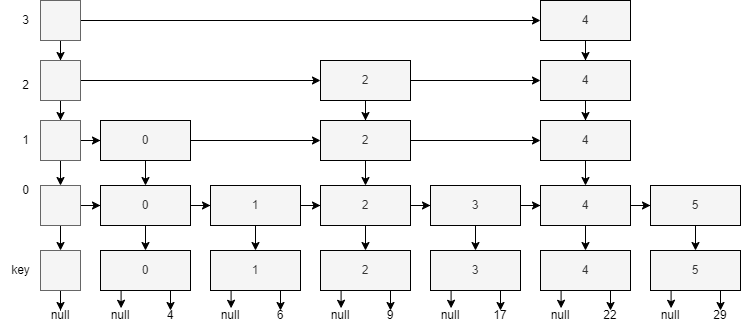
\includegraphics[width=\textwidth]{t1-5.png}
  \end{figure}


  \item Dado un valor $x$, obtener la cantidad de elementos en $L$ menores a $x$.
  Modificar los nodos para almancenar el nodo anterior (atributo \texttt{prev}), de forma que sabremos que el nodo actual es el último por que el apuntador de siguiente apunta a null, y podemos identificar al primero porque su apuntador de \texttt{prev} apunta al placeholder (la columa de nodos que nos indica el nivel) si el \texttt{key,next,down,prev=null}

  De manera que podemos realizar la búsqueda del valor $x$, luego desplazarse al anterior por el atributo \texttt{prev} aumentando un contador hasta encontrar el primer nodo y regresar el contador.


  \begin{figure}[!h]
    \centering
    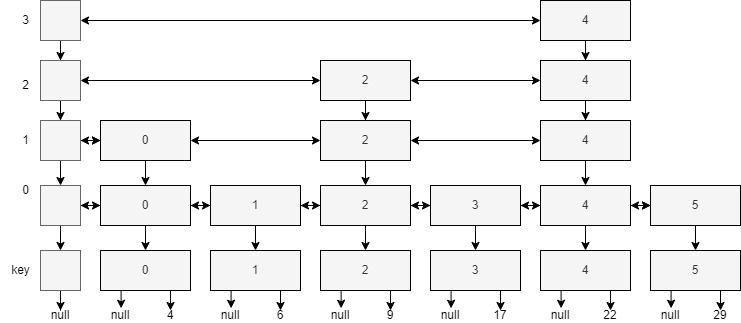
\includegraphics[width=\textwidth]{t1-6.jpg}
    
  \end{figure}

  \end{itemize}

\bigskip
